\documentclass[]{report}
\usepackage{amsmath, amsfonts}
\usepackage{graphicx, subcaption}

% Title Page
\title{MA5678 Assignment: Stage 2}
\author{David Blair}

\newcommand{\real}{\mathbb{R}}
\def\incode#1{\texttt{#1}}

\begin{document}
	\maketitle
	
	\section{Advection (Transport) Equation}
	The advecton equation is as follows:
	\begin{align}
		\frac{\partial u}{\partial t} + c \frac{\partial u}{\partial x} = 0
	\end{align}
	Defined on the domain $ \real \times [0, \infty] $ with initial condition $ u(x, 0) = f(x) $. A solution to this equation is $ u(x, t) = f(x - ct) $:
	\begin{align}
		\frac{\partial u(x, t)}{\partial t} = \frac{\partial f(x - ct)}{\partial t} = -c f^\prime(x - ct) \nonumber \\
		\frac{\partial u(x, t)}{\partial x} = \frac{\partial f(x - ct)}{\partial x} = f^\prime(x - ct) \nonumber \\ \nonumber \\
		-c f^\prime(x - ct) + cf^\prime(x - ct) = 0 \nonumber \\ \nonumber \\ \nonumber 
		u(x, 0) = u(x, 0) = f(x - (0)t) = f(x)
	\end{align}
	A fully commented program to solve this equation numerically using finite differences on a fixed interval $ [x_{min}, x_{max}] \subset \real$ can be found in \incode{transport.m}.
	
	The script \incode{TransportPlot.m} has been modified. Instead of plotting 4 different cross-sectional plots, it plots a 3D graph to illustrate all the data on one plot. You can run this by running the file \incode{main.m}. You can change the function to one of the three variables \incode{f0}, \incode{f1} or \incode{f2}. 
	
	Below are some plots for each of the functions \incode{f0}, \incode{f1} and \incode{f2}. 
	\\\\
	\begin{tabular}{|c|c|c|}
		\hline
		$ f(x) $ & Side View & Top Down  \\
		\hline 
		$ f(x) = sin(\pi x) $ & 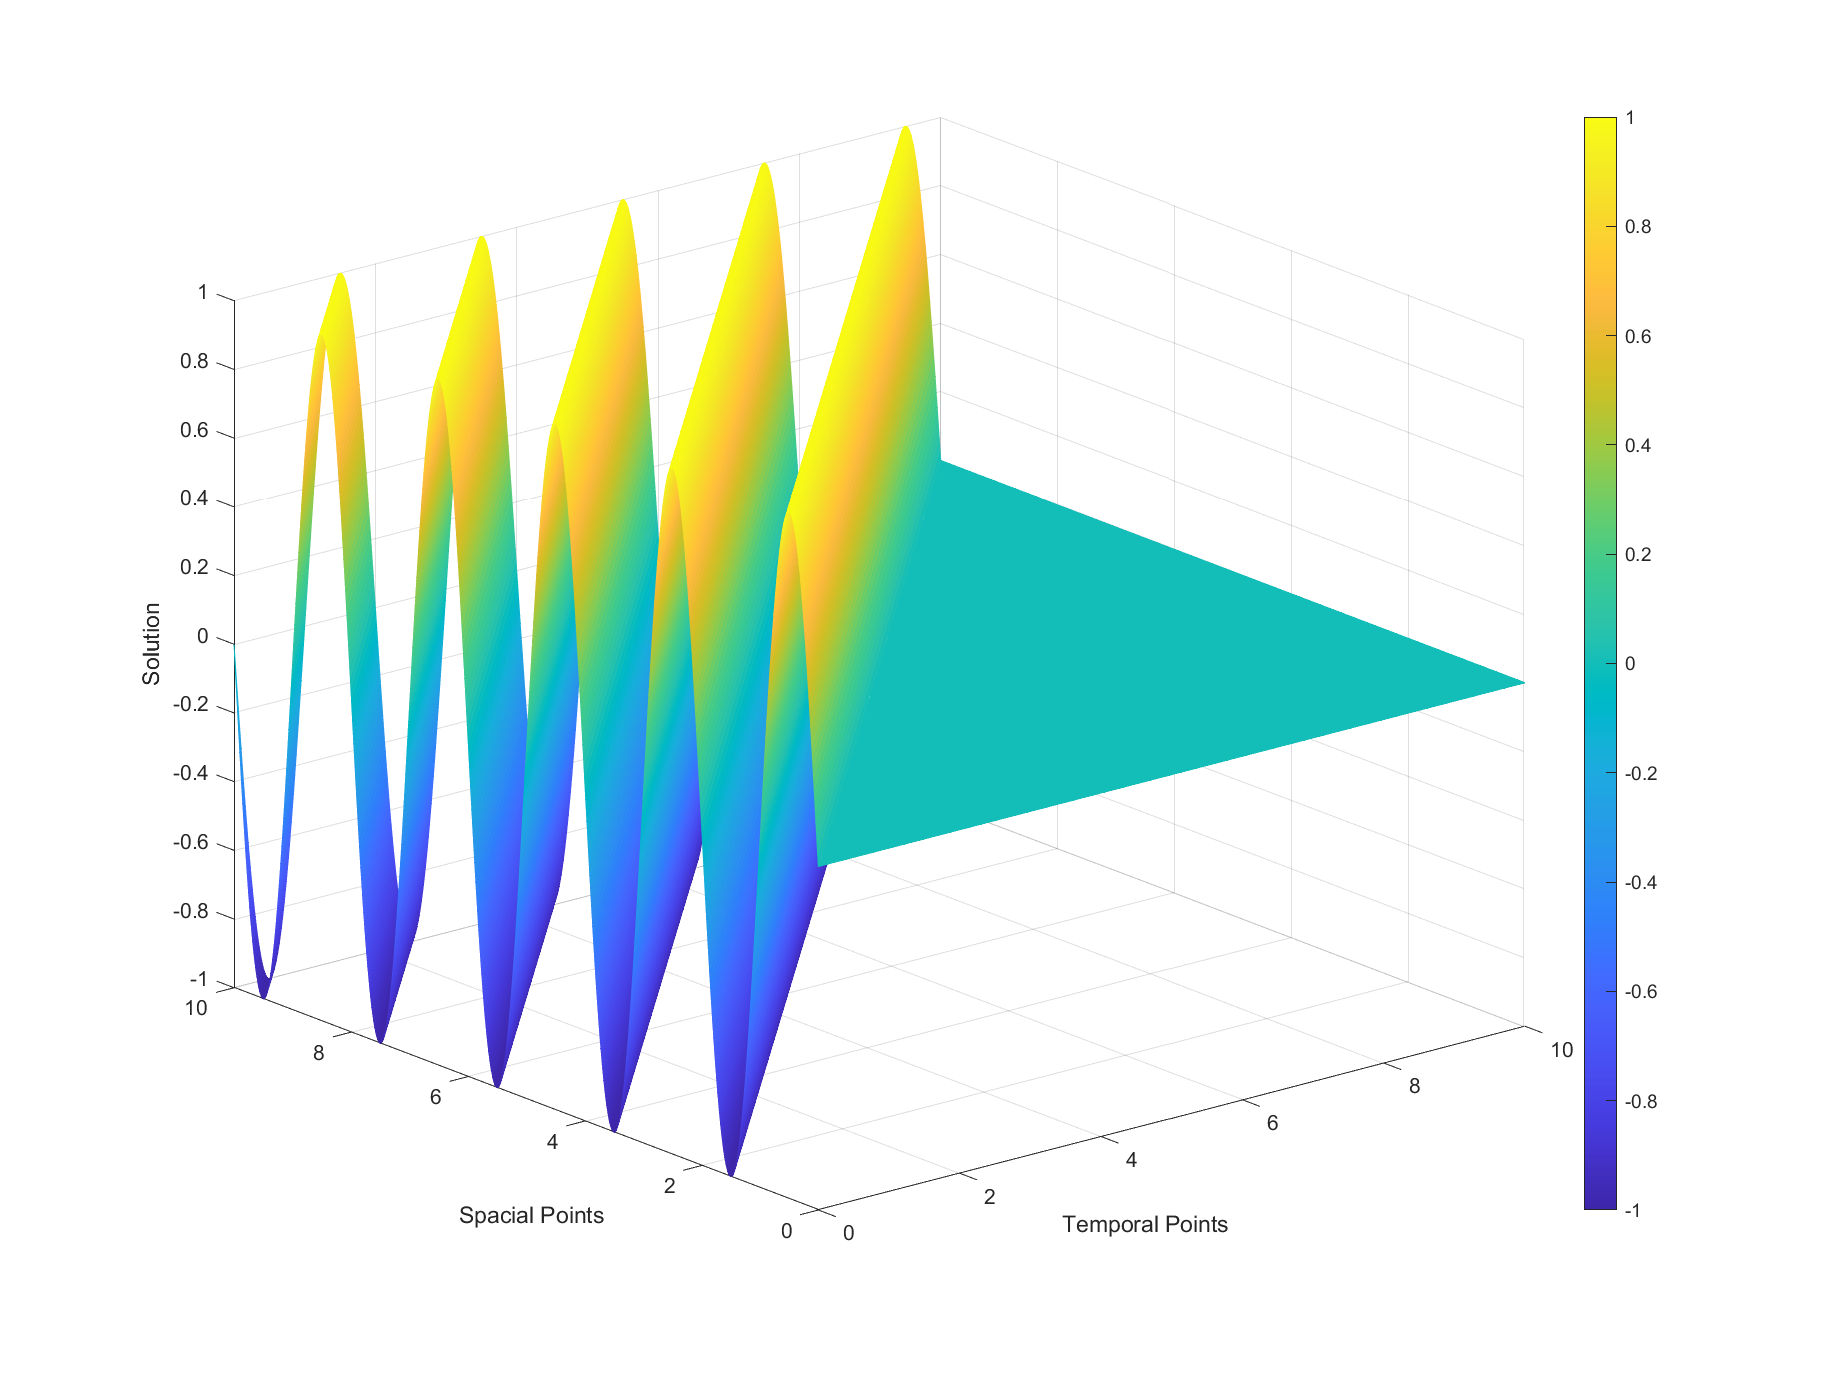
\includegraphics[width=3.6cm]{transport/f0_side.eps} & 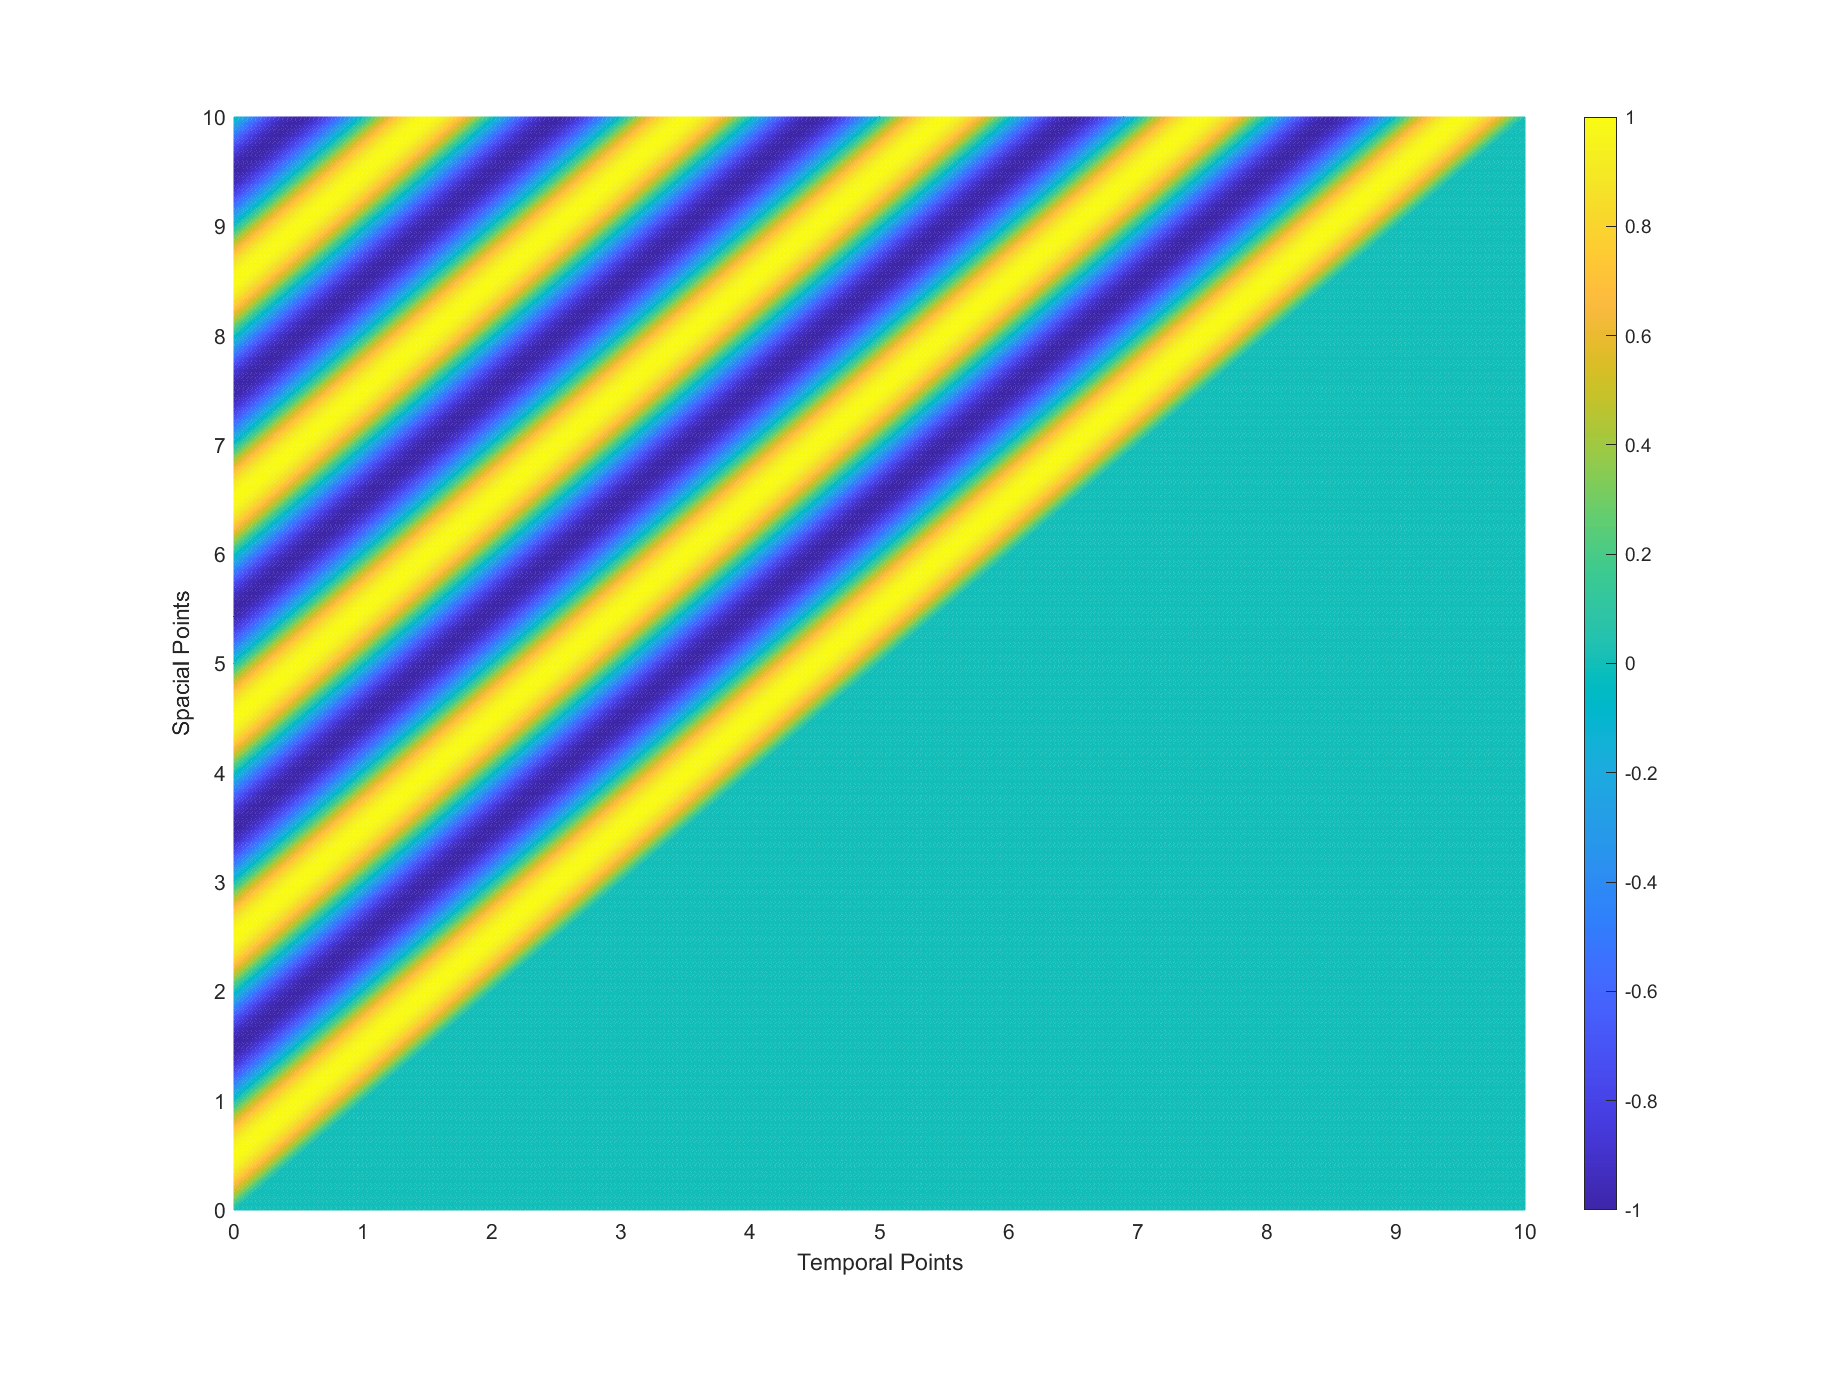
\includegraphics[width=3.6cm]{transport/f0_top.eps} \\
		\hline
		$ f(x) = x^2 $ & 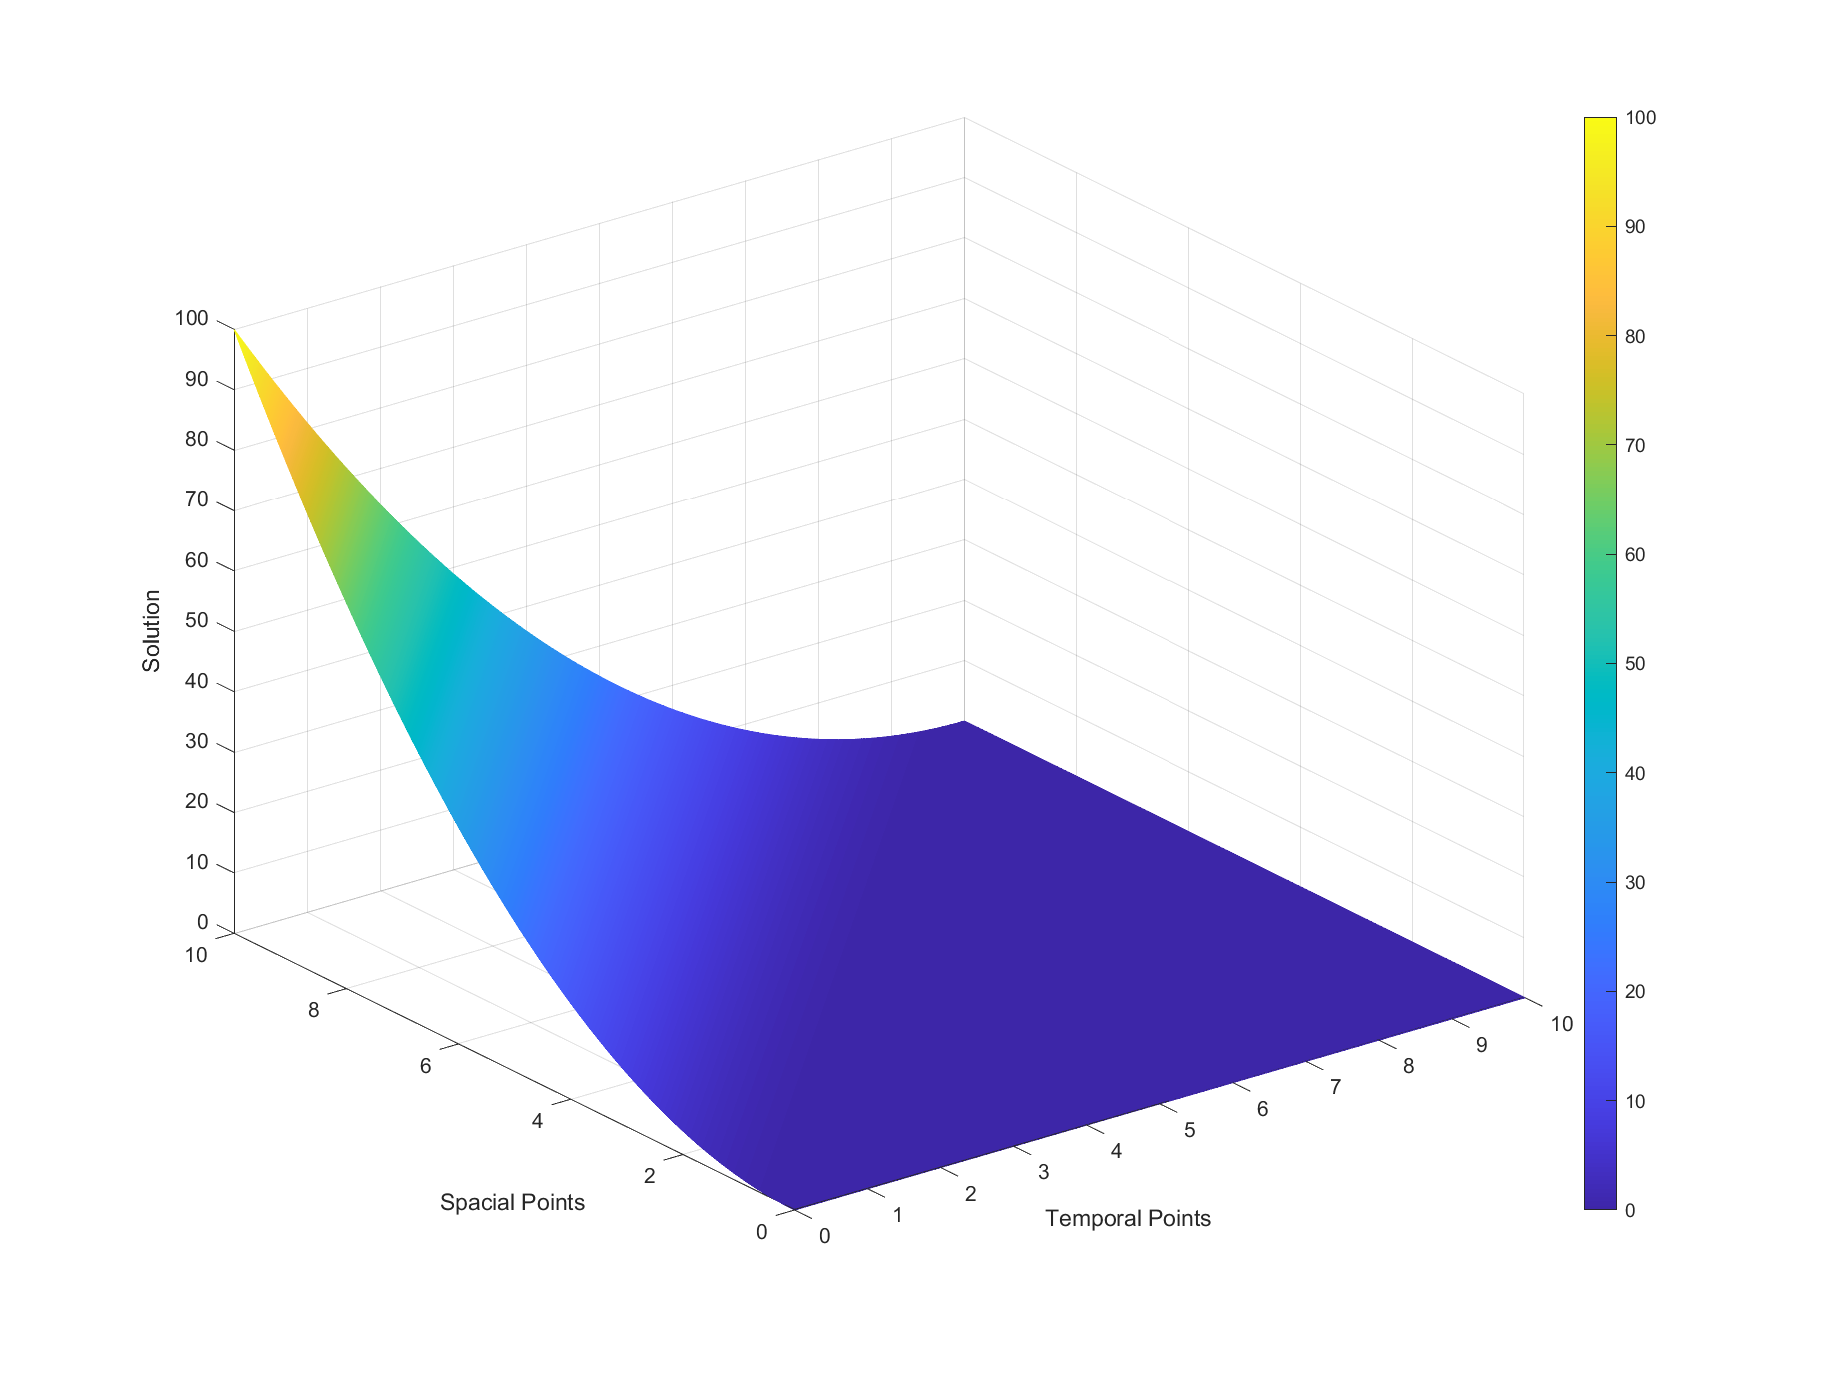
\includegraphics[width=3.6cm]{transport/f1_side.eps} & 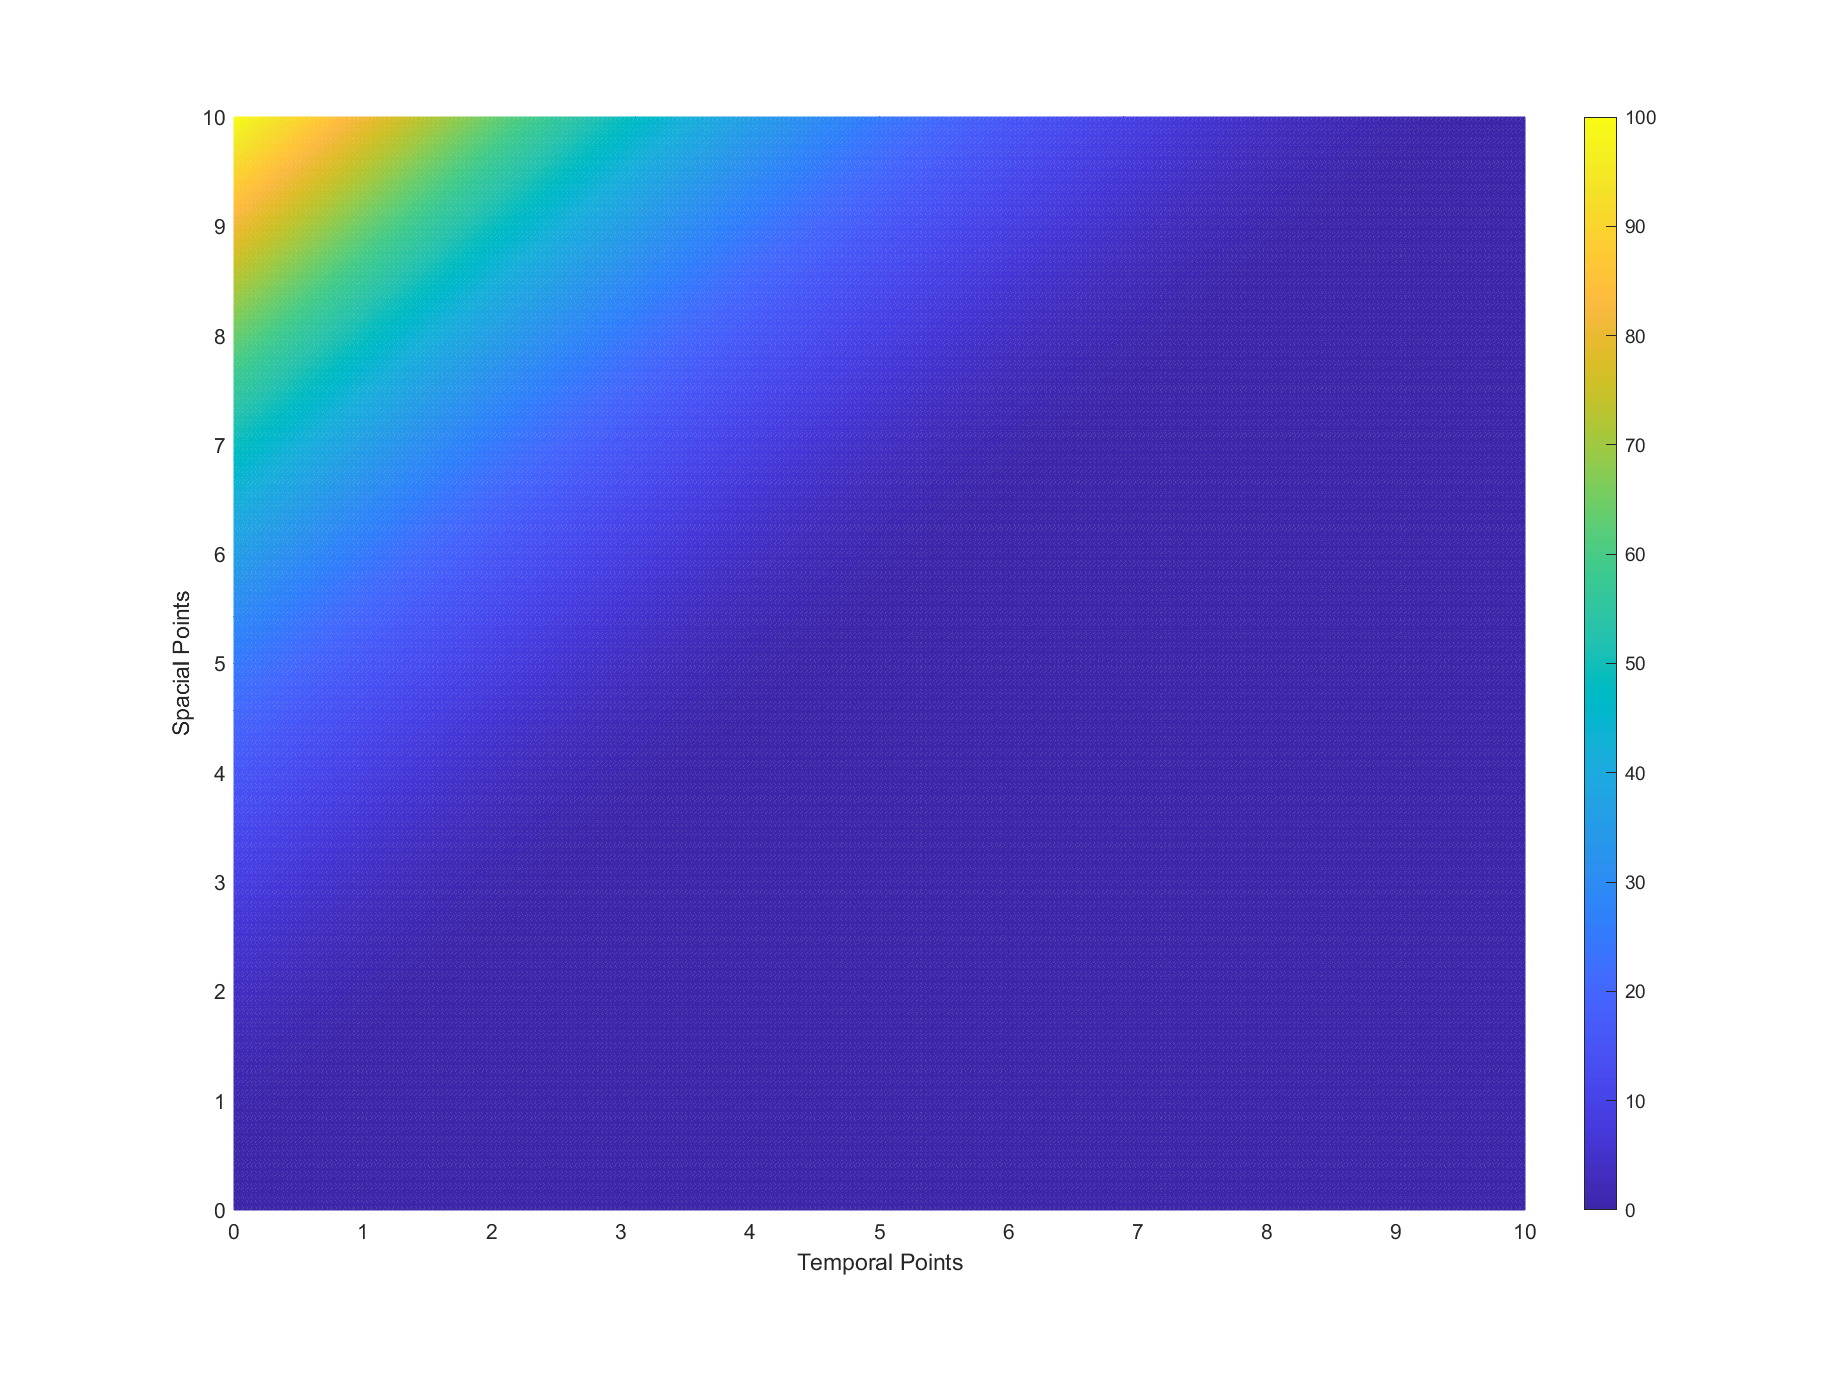
\includegraphics[width=3.6cm]{transport/f1_top.eps}  \\
		\hline
		 $ f(x) = |x| $ & 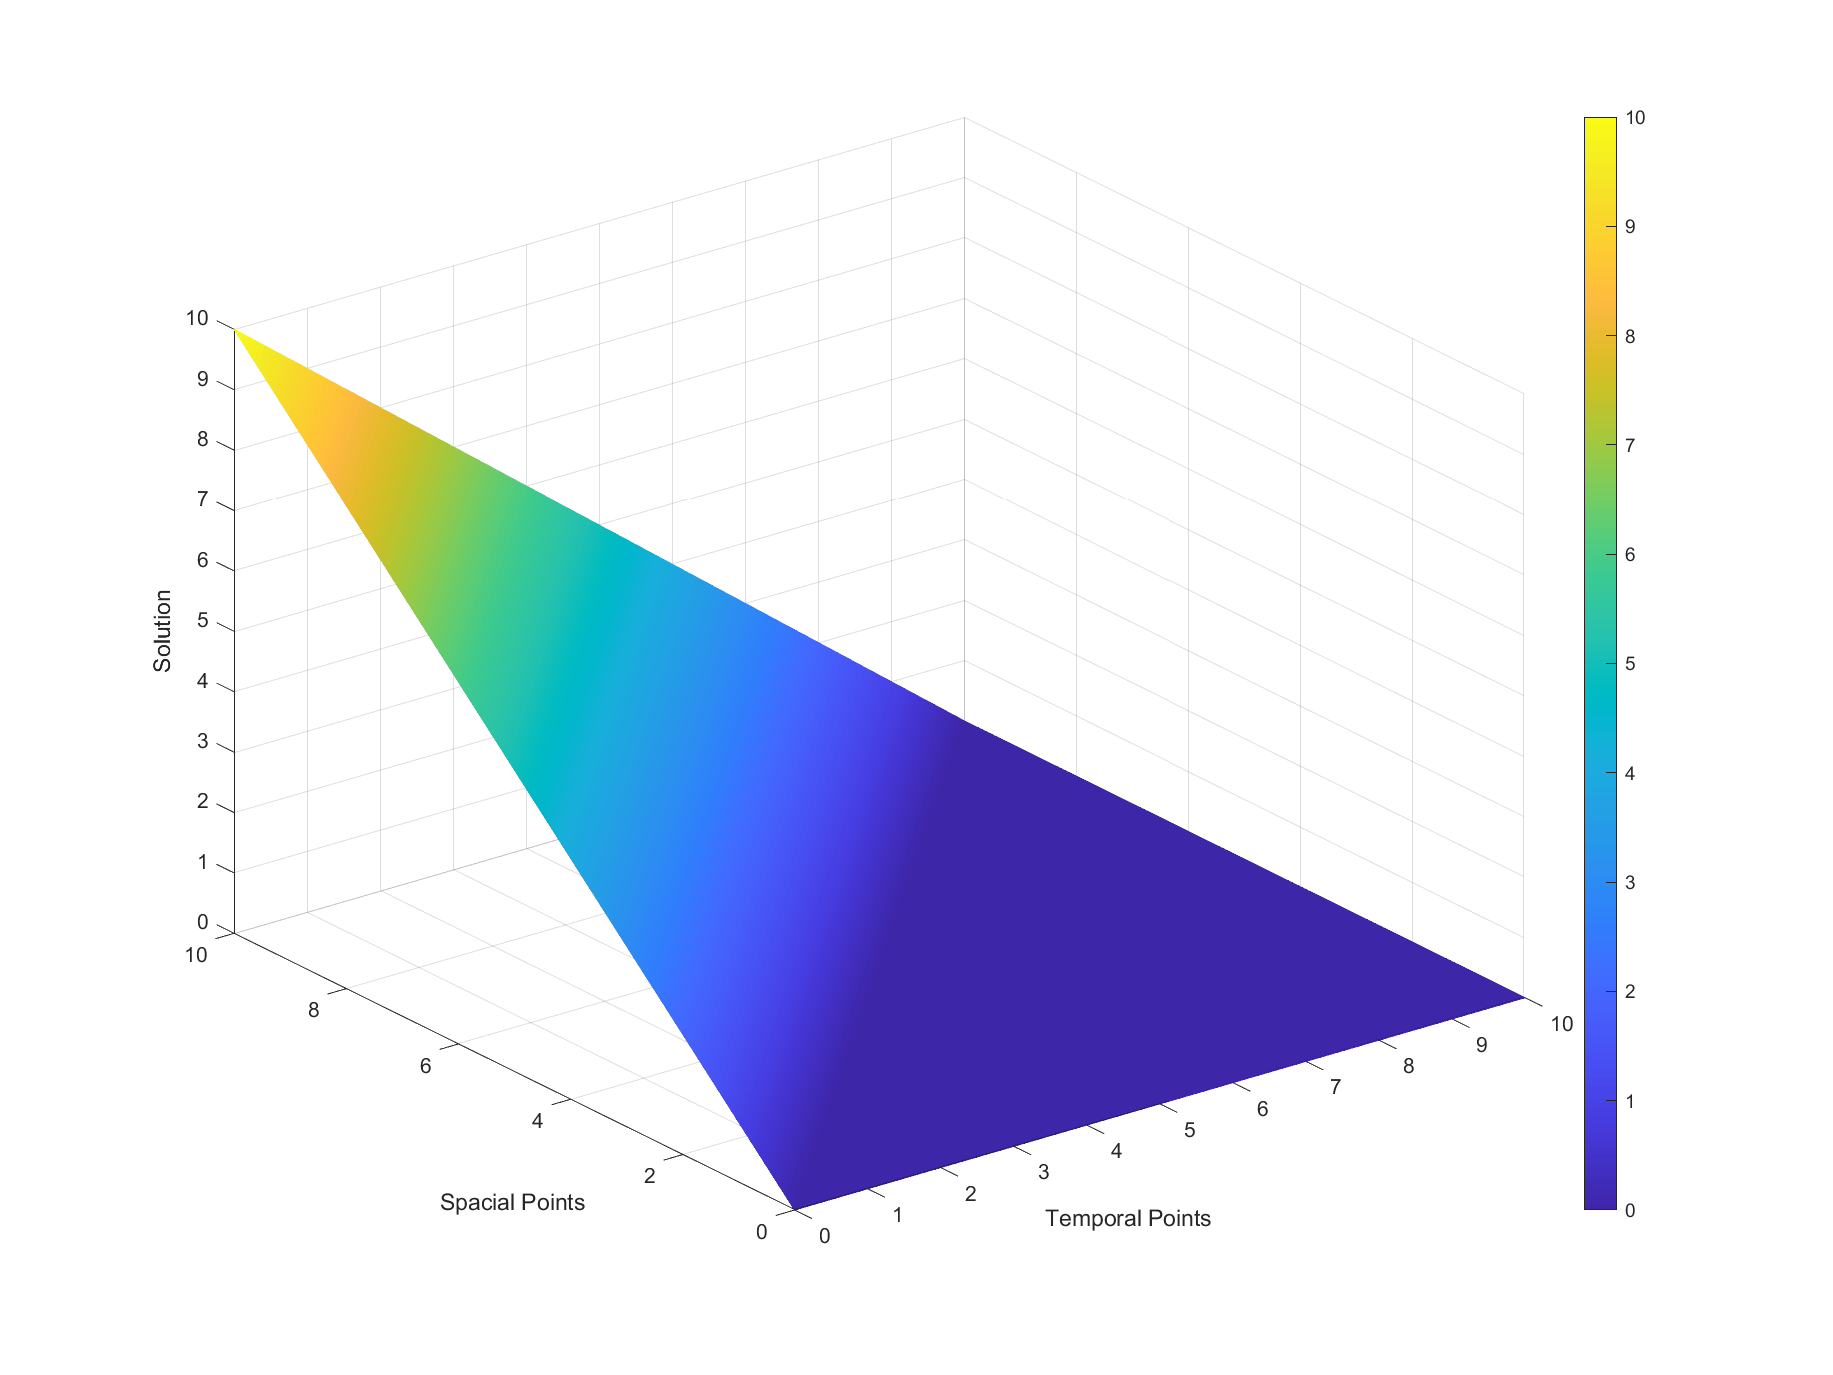
\includegraphics[width=3.6cm]{transport/f2_side.eps} & 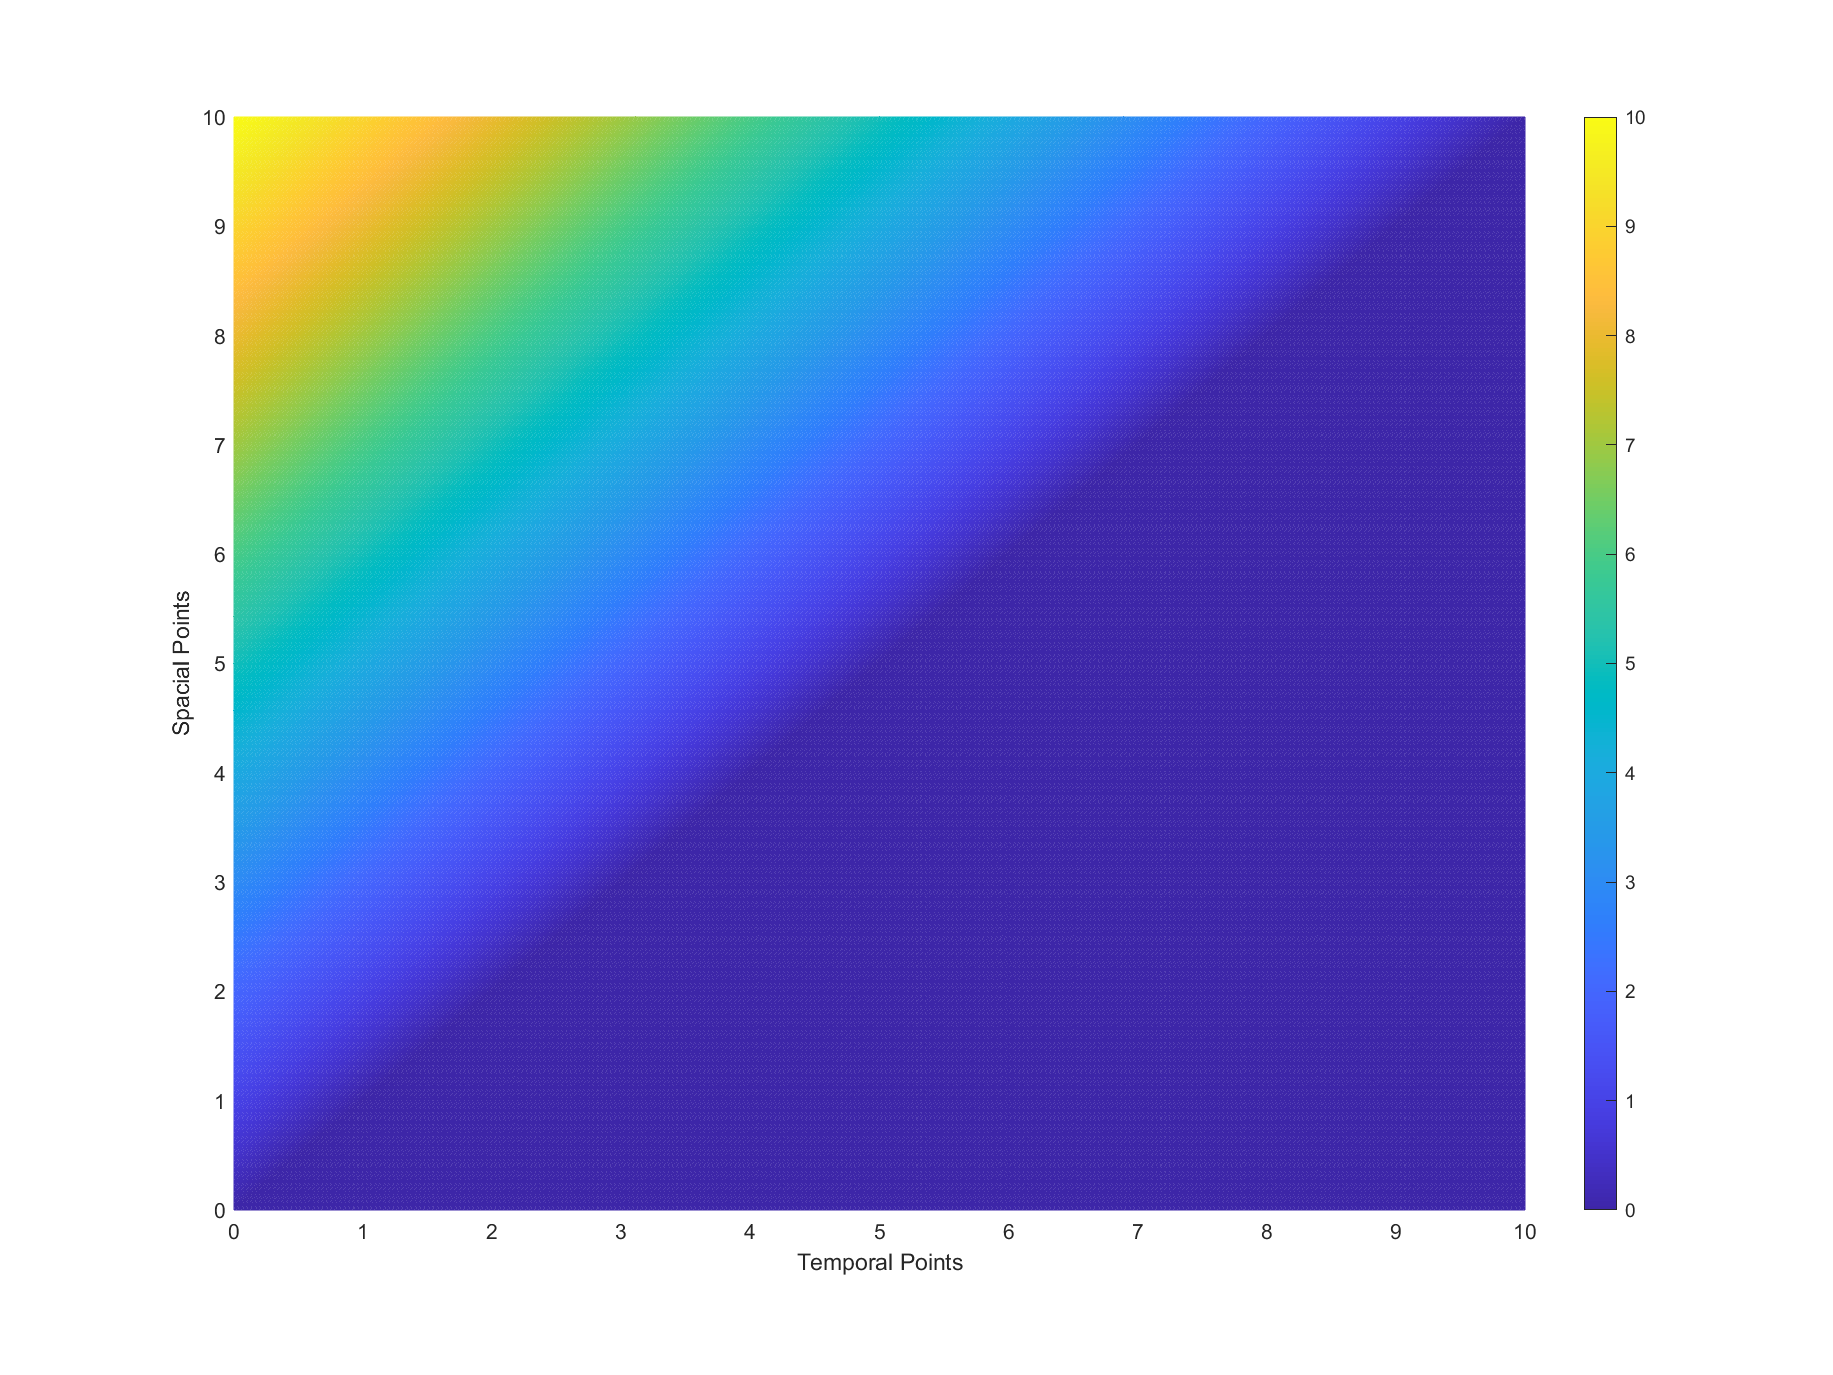
\includegraphics[width=3.6cm]{transport/f2_top.eps}  \\
		\hline
	\end{tabular}

	Below are some solutions to the heat equation for the following parameters: \incode{dt = 0.01}, \incode{dx = 0.02}, \incode{dy = 0.02}, \incode{Tmax = 1}, \incode{Tsnap = [0.25, 0.5, 0.75, 1]}, \incode{value = 1} and \incode{bounds = [0.3, 0.7, 0.3, 0.7]}. \\\\
	
	\begin{tabular}{|c|c|}
		\hline
		time (t) & Solution \\
		\hline
		t = 0 & 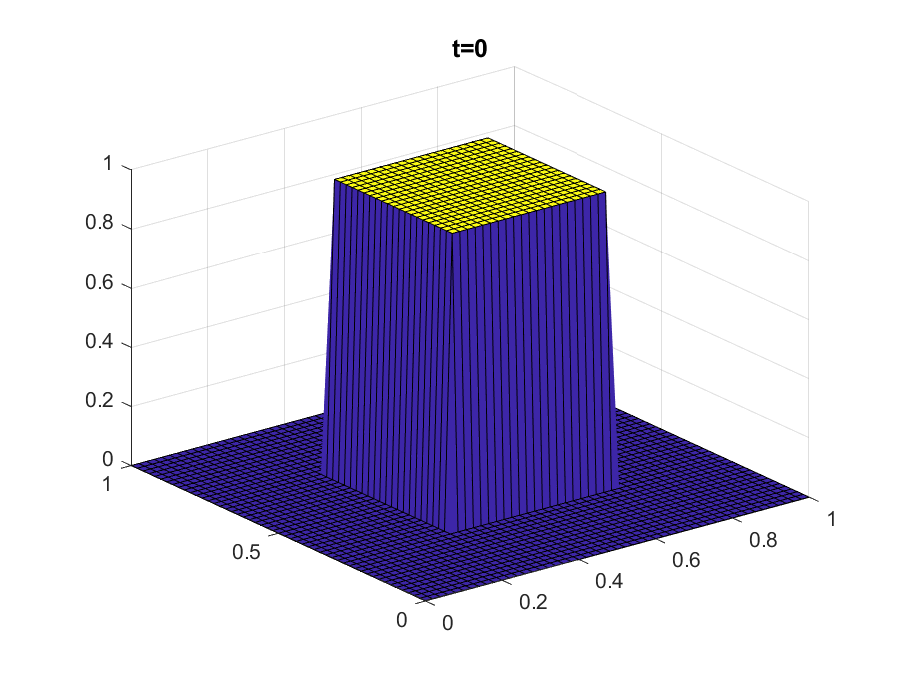
\includegraphics[width=4cm]{heat/h1_t0.eps} \\
		\hline
		t = 0.25 & 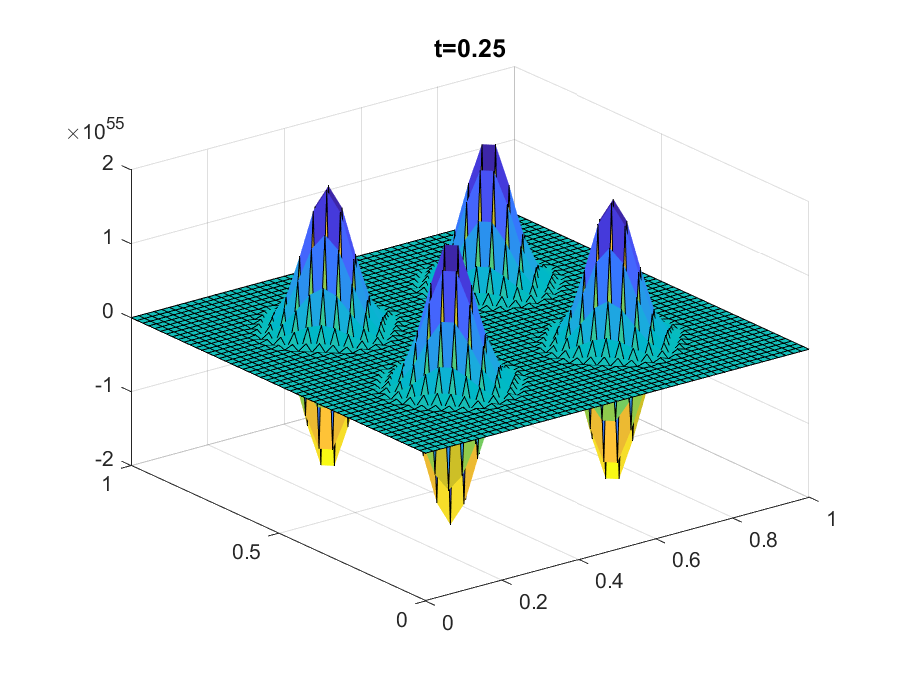
\includegraphics[width=4cm]{heat/h1_t1.eps} \\
		\hline
		t = 0.5 & 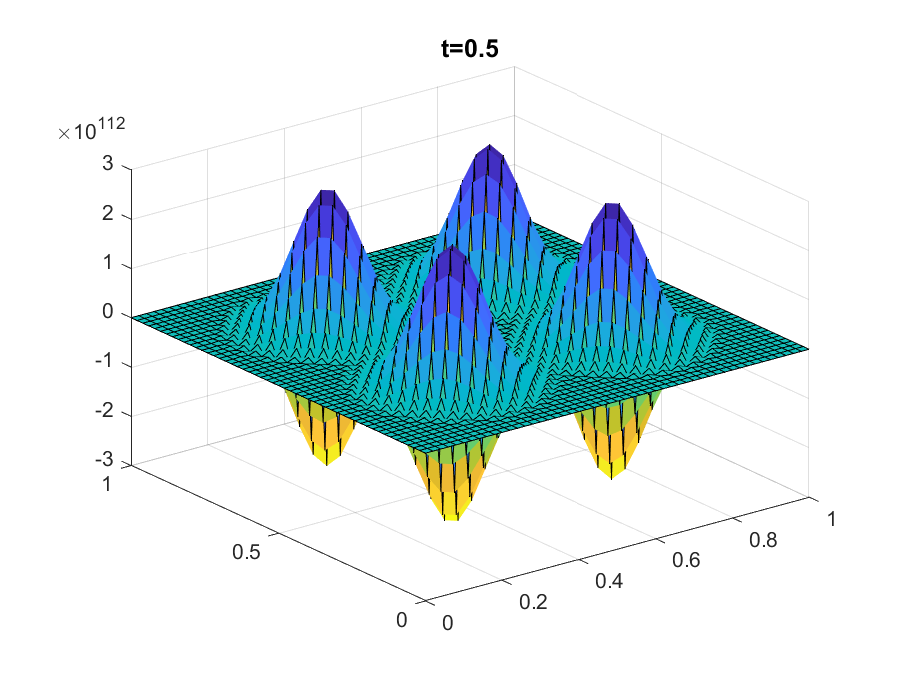
\includegraphics[width=4cm]{heat/h1_t2.eps} \\
		\hline
	\end{tabular}
	\begin{tabular}{|c|c|}
		\hline
		time (t) & Solution \\
		\hline
		t = 0.75 & 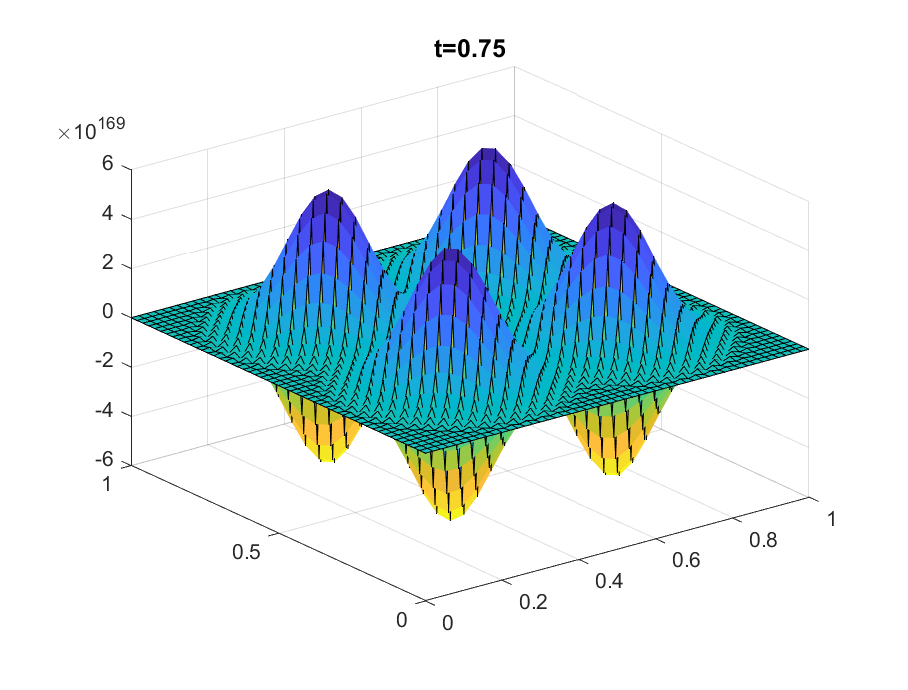
\includegraphics[width=4cm]{heat/h1_t3.eps} \\
		\hline
		t = 1 & 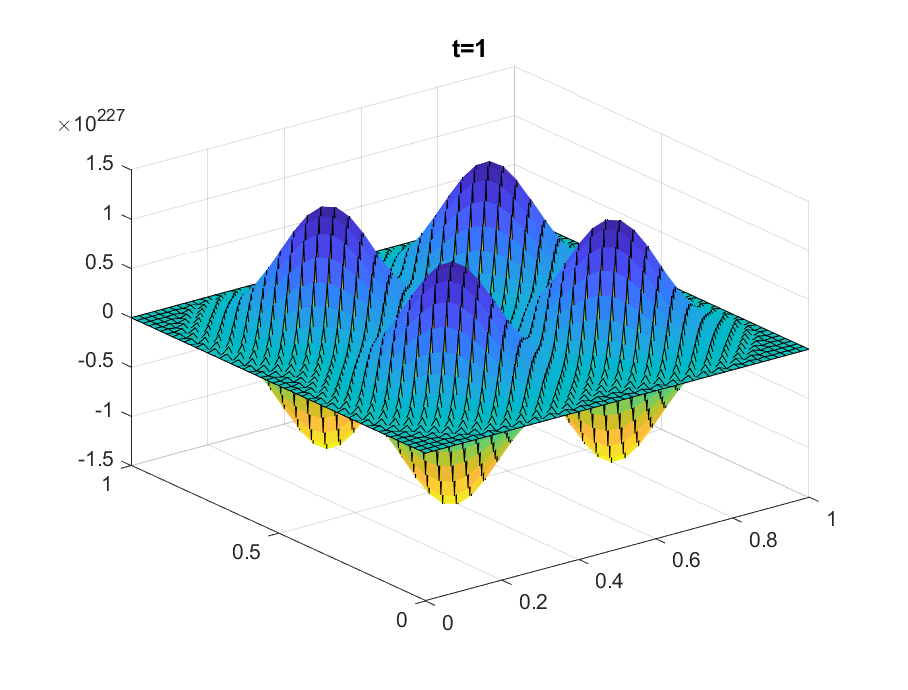
\includegraphics[width=4cm]{heat/h1_t4.eps} \\ 
		\hline
	\end{tabular} 
		\newpage 
		Below are some solutions to the heat equation for the following parameters: \incode{dt = 0.001}, \incode{dx = 0.1}, \incode{dy = 0.1}, \incode{Tmax = 10}, \incode{Tsnap = [1, 2, 4, 6, 8, 10]}, \incode{value = 5} and \incode{bounds = [0.1, 0.9, 0.1, 0.9]}. \\\\
	
	\begin{tabular}{|c|c|}
		\hline
		time (t) & Solution \\
		\hline
		t = 0 & 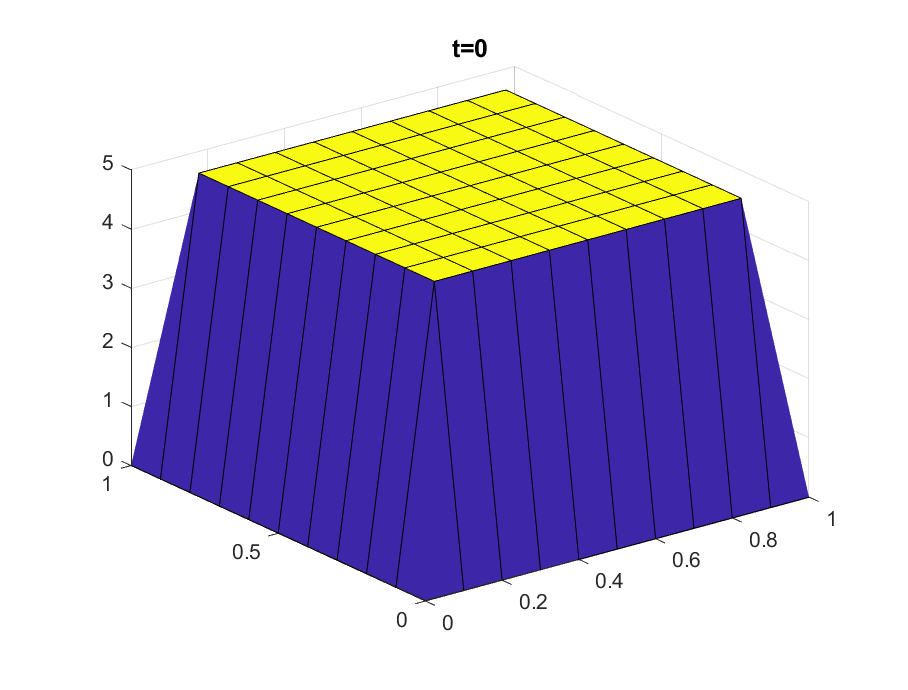
\includegraphics[width=4cm]{heat/h2_t0.eps} \\
		\hline
		t = 1 & \includegraphics[width=4cm]{heat/h2_t1.eps} \\
		\hline
		t = 2 & 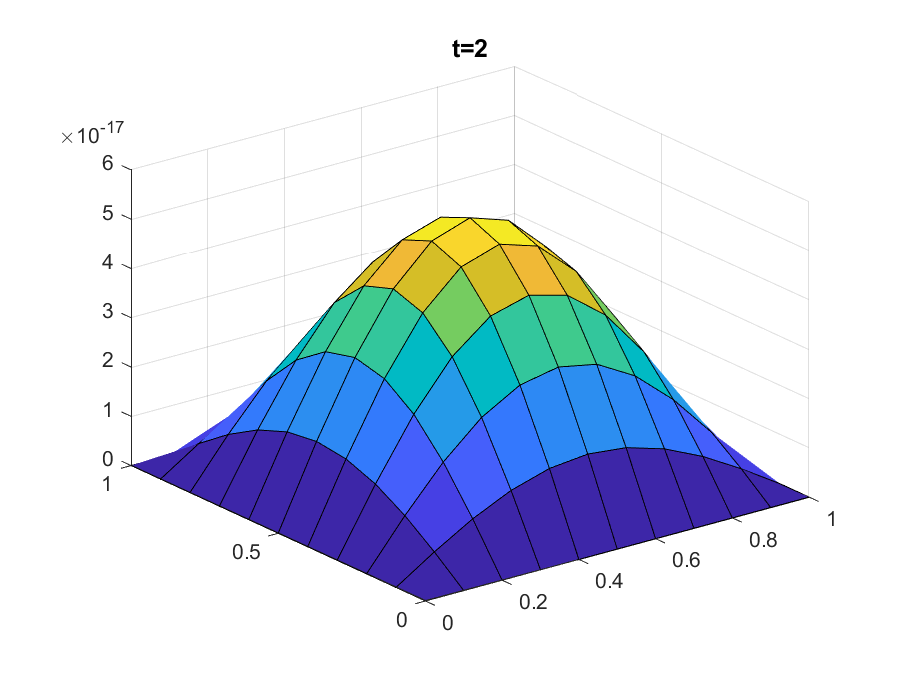
\includegraphics[width=4cm]{heat/h2_t2.eps} \\
		\hline
		t = 4 & 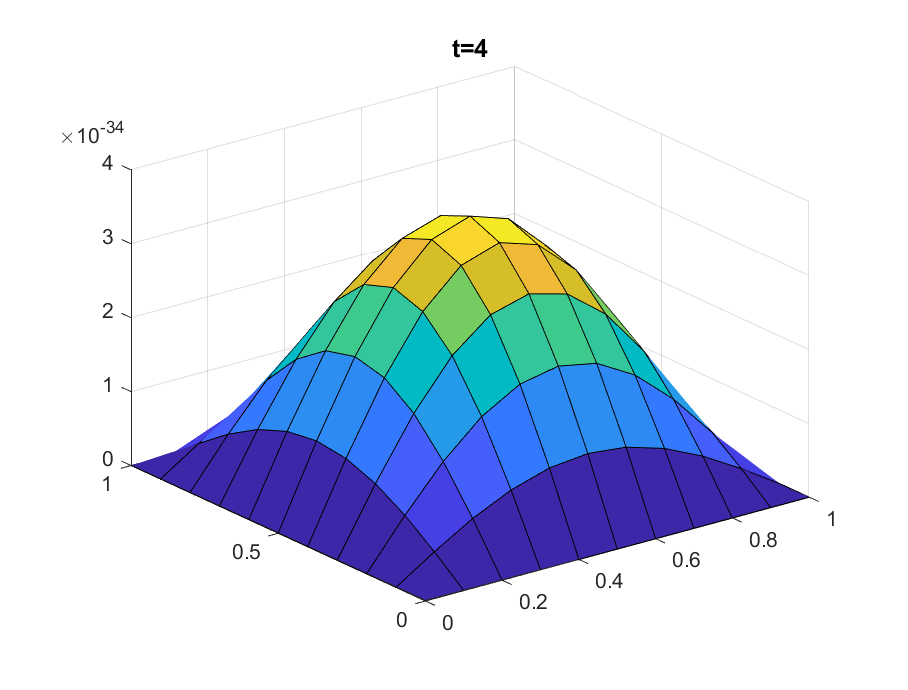
\includegraphics[width=4cm]{heat/h2_t3.eps} \\
		\hline
	\end{tabular}
	\begin{tabular}{|c|c|}
		\hline
		time (t) & Solution \\
		\hline
		t = 6 & 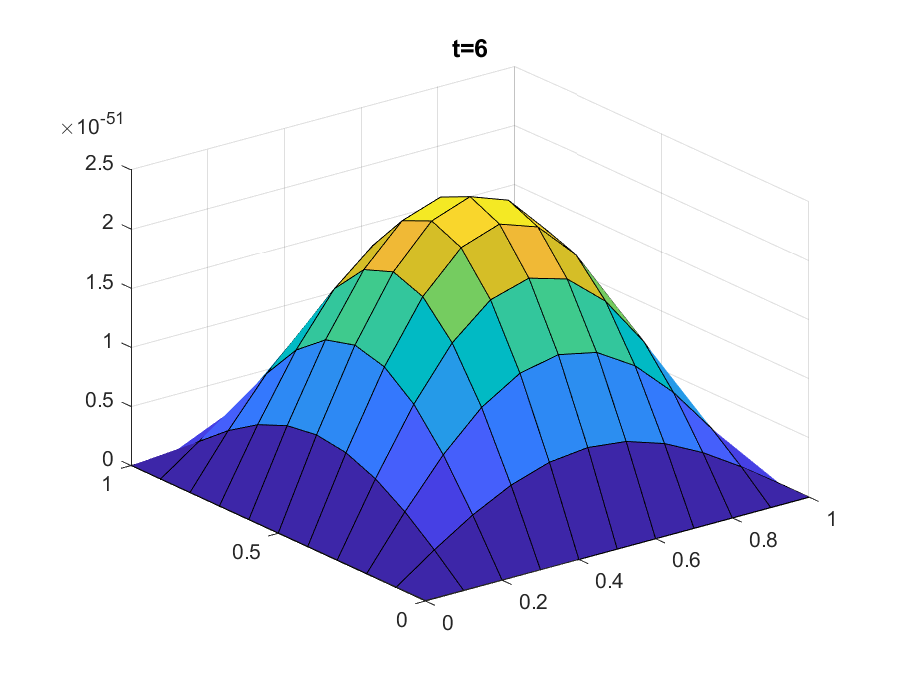
\includegraphics[width=4cm]{heat/h2_t4.eps} \\
		\hline
		t = 8 & 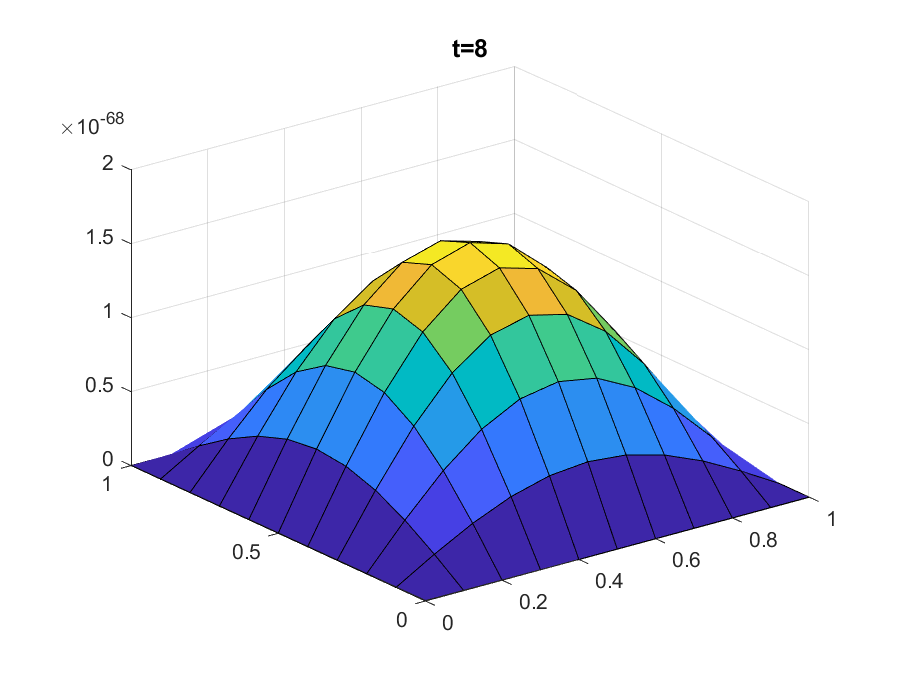
\includegraphics[width=4cm]{heat/h2_t5.eps} \\
		\hline
		t = 10 & 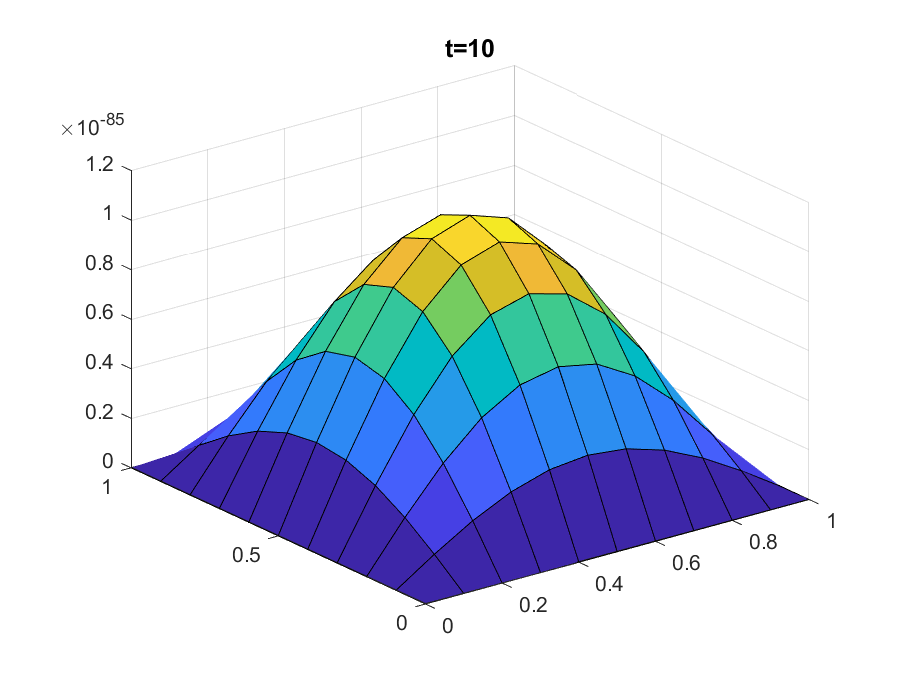
\includegraphics[width=4cm]{heat/h2_t6.eps} \\
		\hline
	\end{tabular}
	In \incode{Heat2D\_modified.m} you'll find a version of the original code where we have added a heat sink at coordinates $(0.1, 0.1)$. You can modify the value of \incode{alpha} to get varying strengths, a higher alpha value meaning a greater sink of heat. 
	\section{Task 3}
	This section is concerned with the Insect Dispersal Model
	
	\begin{align}
		n_t &= d_0 \left( \left(\frac{n}{n_0}\right)^m n_x \right)_x \\
		&= \frac{d}{n_{0}^m} \left( n^m n_x \right)_x \\
		&= \frac{d}{n_{0}^m} \left( mn^{n - 1} (n_x)^2 + n^m n_{xx} \right) \\
		&= \frac{dn^{m - 1}}{n_{0}^m} \left( m(n_x)^2 + nn_{xx} \right) \\ \nonumber \\
		n_{xx} &\approx \frac{n_{i + 1, j} + n_{i - 1, j} -2n_{i, j}}{(\Delta x)^2} \\ \nonumber \\
		n_x &\approx \frac{n_{i + 1, j} - n_{i - 1, j}}{2(\Delta x)} \\ \nonumber \\
		n_t &\approx \frac{n_{i, j + 1} - n_{i, j}}{\Delta t} \\ \nonumber \\
		n_x&(-x, t) = n_x(x, t) = 0 \\ n_x &= 0 \nonumber \\ n(0, 0) &= 0 \nonumber \\ \nonumber \\
	\end{align}
\end{document}